\documentclass{scrreprt}   % instead of  \documentclass[a4paper]{article}
%\usepackage{graphicx}
% the following style (can also be included by copy and paste)
% tries to mimic the Framemaker layout used by the OMG standards,
% i.e.:
% - paper size 8.28x11 inch
% - text size 6.7x8in
% - times roman, helvetica, and courier as fonts
% - ragged right paragraph formatting
\usepackage{omg}
%\usepackage{url}
%\usepackage{pifont}
\usepackage{upquote}
\usepackage{alltt}
\usepackage{graphicx}

\begin{document}

\oclHeadingOne{Scope}
\oclHeadingOne{Conformance}
\oclHeadingOne{Normative References}
\oclHeadingOne{Terms and Definitions}
\oclHeadingOne{Symbols}
\oclHeadingOne{Additional Information}

\oclHeadingOne{Abstract Syntax}\label{ocl:AbstractSyntax}
\oclHeadingTwo{Pivot Abstract Syntax Model}
\input{../latex-gen/abstract-syntax}

\oclHeadingOne{Concrete Syntax}\label{ocl:ConcreteSyntax}

This clause describes the concrete syntax of the OCL. This allows modelers to write down OCL expressions in a standardized way. The trnasformation from the normative textual concrete syntax via a non-normative concrete syntax model to the normative absract syntax involves the conversions shown in Figure \ref{ocl:Conversions}.

\begin{figure}
  \begin{center}
    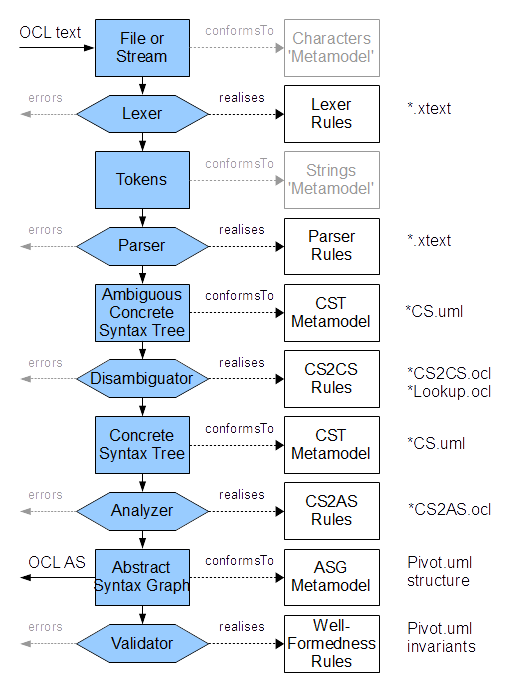
\includegraphics[width=4.5in]{Conversions.png}
  \end{center}
  \centering
%  \centerline{\Large\textbf{Example Figure}}
  \caption{This is an example figure caption}\label{ocl:Conversions}
\end{figure}

The source text characters are grouped into tokens by the lexer. The grammar is unfortunately not amenable to an unambiguous parse and so the parser result is an ambiguous concrete syntax tree. The disambiguator produces the unambiguous concrete syntax tree that the analyzer converts to the abstract syntax graph. The validator diagnoses well-formedness violations.

With the exception of the trivial characters and tokens representations, each representation conforms to a metamodel, grammar and eacg conversion realizes rules defined in this specification.

\begin{itemize}
\item The lexer realizes the Lexer Rules defined in this clause and Base.xtext, EssentialOCL.xtext and CompleteOCL.xtext.
\item The parser realizes the Parser Rules defined in this clause and Base.xtext, EssentialOCL.xtext and CompleteOCL.xtext.
\item Parser. The parser realizes the Parser Rules defined in this clause and Base.xtext, EssentialOCL.xtext and CompleteOCL.xtext.
\item The disambiguator perforns a CS to CS conversion replacing ambiguous CS elements by unambiguous CS elements. The disambiguation rules are provided in this clause and EssentialOCLCS2CS.ocl. Resolution of names are provided in ... and PivotLookup.ocl.
\item The analyzer performs a CS to AS conversion from unambiguous CS elements to AS elements. The conversion rules are provided in this clause and BaseCS2AS.ocl, EssentialOCLCS2AS.ocl, CompleteOCLCS2AS.ocl. Resolution of names are provided in ... and PivotLookup.ocl.
\item The validator performs an AS validity check using well-formedness rules embedded as constraints in the Abstract Syntax metamodel.
\item The Concrete Syntax Metamodel provides example classes for the non-normative intermediate representations created by the parser, refined by the disambiguator and used by the analyzer.  The CS is defined by BaseCS.uml, EssentialOCLCS.uml, CompleteOCLCS.uml.
\item The Abstract Syntax Metamodel defines the normative representations created by the analyzer and used for XMI interchange.  The AS is defined by Pivot.uml.
\end{itemize}

%A formal mapping from the concrete syntax to the abstract syntax from Clause \ref{ocl:AbstractSyntax} ``Abstract Syntax'' is given. Although not required, sub clause 9.6 describes a mapping from the abstract syntax to the concrete syntax. This allows one to produce a standard human readable version of any OCL expression that is represented as an instance of the abstract syntax. Sub clause \ref{ocl:ConcreteSyntax:Structure} ``Structure of the Concrete Syntax'' describes the structure of the grammar and the motivation for the use of an attribute grammar.

\oclHeadingTwo{Structure of the Concrete Syntax}\label{ocl:ConcreteSyntax:Structure}
The concrete syntax of OCL is described using an Annotated Extended Backus-Naur Form grammar whose syntax is defined in Clause \ref{ocl:AnnotatedEBNF}.

The concrete syntax is partitioned into Base OCL, Essential OCL and Complete OCL modules and further partitioned by the produced CS classes. The parser rules that produce each CS class are grouped together wih annotations to show how the ambiguous CS is populated. For ambiguous CS classes, CS2CS disambiguation rules define the disambiguation. For unambiguous CS classes, CS2AS rules define the mapping to the AS. For all CS classes attributes, associations and superclasses are identified.

%Each production in an attribute grammar may have synthesized attributes attached to it. The value of synthesized attributes of elements on the left hand side of a production rule is always derived from attributes of elements at the right hand side of that production rule. Each production may also have inherited attributes attached to it. The value of inherited attributes of elements on the right hand side of a production rule is always derived from attributes of elements on the left hand side of that production. In the attribute grammar that specifies the concrete syntax, every production rule is denoted using the EBNF formalism and annotated with synthesized and inherited attributes, and disambiguating rules. There are a number of special annotations, as follows.
\oclHeadingZero{Synthesized Attributes}
Each production rule has one synthesized attribute called ast (short for abstract syntax tree), that holds the instance of the
OCL Abstract Syntax that is returned by the rule. The type of ast is different for every rule, but it always is an element of
the abstract syntax. The type is stated with each production rule under the heading “Abstract Syntax Mapping.” The ast
attribute constitutes the formal mapping from concrete syntax to abstract syntax.
The motivation for the use of an attribute grammar is the easiness of the construction and the clarity of this mapping.
Note that each name in the EBNF format of the production rule is postfixed with ‘CS’ to clearly distinguish between the
concrete syntax elements and their abstract syntax counterparts.
\oclHeadingZero{Inherited Attributes}
Each production rule has one inherited attribute called env (short for environment), that holds a list of names that are
visible from the expression. All names are references to elements in the model. In fact, env is a name space environment
for the expression or expression part denoted according to the production rule. The type of the env attribute is
Environment, as shown in Figure 9.1. A number of operations are defined for this type. Their definitions and more details
on the Environment type can be found in sub clause 9.4. The manner in which both the ast and env attributes are
determined is given using OCL expressions.

Note that the contents of the env attribute are fully determined by the context of the OCL expression. When an OCL
expression is used as an invariant to class X, its environment will be different than in the case the expression is used as a
postcondition to an operation of class Y. In Clause 12 (“The Use of Ocl Expressions in UML Models”) the context of
OCL expressions is defined in detail.
\oclHeadingZero{Multiple Production Rules}
For some elements there is a choice of multiple production rules. In that case the EBNF format of each production rule is
prefixed by a capital letter between square brackets. The same prefix is used for the corresponding determination rules for
the ast and env attributes.
\oclHeadingZero{Multiple Occurrences of Production Names}
In some production rules the same element name is used more than once. To distinguish between these occurrences the
names will be postfixed by a number in square brackets, as in the following example.
CollectionRangeCS ::= OclExpressionCS[1] ‘..’ OclExpressionCS[2]
\oclHeadingZero{Disambiguating Rules}
Some of the production rules are syntactically ambiguous. For such productions disambiguating rules have been defined.
Using these rules, each production and thus the complete grammar becomes nonambiguous. For example in parsing a.b(),
there are at least three possible parsing solutions:
1. a is a VariableExpr (a reference to a let or an iterator variable)
2. a is an AttributeCallExp (self is implicit)
3. a is a NavigationCallExp (self is implicit)
A decision on which grammar production rule to use can only be made when the environment of the expression is taken
into account. The disambiguating rules describe these choices based on the environment and allow unambiguous parsing
of a.b(). In this case the rules (in plain English) would be:
• If a is a defined variable in the current scope, a is a VariableExp.
• If not, check self and all iterator variables in scope. The inner-most scope for which as is either
• an attribute with the name a, resulting in an AttributeCallExp, or
• an opposite association-end with the name a, resulting in a NavigationCallExp, defines the meaning of a.b().
• If neither of the above is true, the expression is illegal / incorrect and cannot be parsed.
Disambiguating rules may be based on the UML model to which the OCL expression is attached (e.g., does an attribute
exist or not). Because of this, the UML model must be available when an OCL expression is parsed, otherwise it cannot
be validated as a correct expression. The grammar is structured in such a way that at most one of the production rules will
fulfill all the disambiguating rules, thus ensuring that the grammar as a whole is unambiguous. The disambiguating rules
are written in OCL, and use some metaclasses and additional operations from UML.

\oclHeadingTwo{A Note to Tool Builders}
\oclHeadingThree{Parsing}
The grammar in this clause might not prove to be the most efficient way to directly construct a tool. Of course, a toolbuilder
is free to use a different parsing mechanism. He can, for example, first parse an OCL expression using a special
concrete syntax tree, and do the semantic validation against a UML model in a second pass. Also, error correction or
syntax directed editing might need hand-optimized grammars. This document does not prescribe any specific parsing
approach. The only restriction is that at the end of all processing a tool should be able to produce the same well-formed
instance of the abstract syntax, as would be produced by this grammar.
\oclHeadingThree{Visibility}
The OCL specification puts no restriction on the visibility declared for a property defined in the model (such as ‘private,’
‘protected,’ or ‘public’). In OCL, all model elements are considered visible. The reason for this is to allow a modeler to
specify constraints, even between ‘hidden’ elements. At the lowest implementation level this might be useful.
As a separate option OCL tools may enforce all UML visibility rules to support OCL expressions to be specified only
over visible model elements. Especially when a tool needs to generate code for runtime evaluation of OCL expressions,
this visibility enforcement is necessary.

\oclHeadingTwo{Base OCL}\label{ocl:BaseOCLConcreteSyntax}
\input{../latex-gen/base-cs}

\oclHeadingTwo{Essential OCL}\label{ocl:EssentialOCLConcreteSyntax}
\input{../latex-gen/essentialocl-cs}

\oclHeadingTwo{Complete OCL}\label{ocl:CompleteOCLConcreteSyntax}
\input{../latex-gen/completeocl-cs}

\oclHeadingTwo{Environment Definition}
The Environment type used in the rules for the concrete syntax is defined according to the following invariants and
additional operations. A diagrammatic view can be found in Figure 9.1. Environments can be nested, denoted by the
existence of a parent environment. Each environment keeps a list of named elements, that have a name a reference to a
ModelElement.

\oclHeadingTwo{Concrete to Abstract Syntax Mapping}
The mapping from concrete to abstract syntax is described as part of the grammar. It is described by adding a synthesized
attribute ast to each production that has the corresponding metaclass from the abstract syntax as its type. This allows the
mapping to be fully formalized within the attribute grammar formalism.

\oclHeadingTwo{Abstract Syntax to Concrete Syntax Mapping}
It is often useful to have a defined mapping from the abstract syntax to the concrete syntax. This mapping can be defined
by applying the production rules in sub clause 9.3 from left to right. As a general guideline nothing will be implicit (for
example, implicit collect, implicit use of object as set) and all iterator variables will be filled in completely. The mapping
is not formally defined in this document but should be obvious.

\oclHeadingOne{Evaluation Semantics}\label{ocl:EvaluationSemantics}
\oclHeadingTwo{Model}
%\input{../latex-gen/evaluation-semantics}

\oclHeadingOne{OCL Standard Library}
This documentation on the OCL Standard Library is auto-generated from the
org.eclipse.ocl.examples.library/model/OCL-2.5.oclstdlib that defines
the behaviour of the Pivot evaluator and the Xtext editors. It is similar to the OCL 2.4 functionality.
It is a prototype of functionality for OCL 2.5 where the use of models may eliminate ambiguities.
		
The library support for the Ecore and UML bindings in Luna has been upgraded so that the available operations
are similar to those documented here for the Pivot binding.
\oclHeadingTwo{Library Model}
\input{../latex-gen/ocl-standard-library}

%\chapter{The Models}
\oclHeadingOne{The Models}\label{ocl:TheModels}

This specification is substantially auto-generated from the normative models that accompany it.

<<<Migrate all *.ecore files to *.xmi>>>

\oclHeadingTwo{The Abstract Syntax (AS)}

The abstract syntax model Pivot.ecore is the result of a merge of UML.xmi and OCL.xmi followed by the QVTo transformations UML2EcoreAnalysis.qvto and UML2EcoreSynthesis.qvto that use the UML2PivotinEcore.xmi control file and UML2EcoreControl.ecore and UML2EcoreMapping.ecore intermeiate representations.

Well-formedness rules are provided by Pivot.ocl and Types.ocl.

Name resolution rules are defined in Lookup.ocl.

\oclHeadingTwo{The Concrete Syntax (CS)}

The non-normative concrete syntax models Base.ecore, EssentialOCL.ecore and CompleteOCL.ecore support the EssentialOCL.xtext and CompleteOCL.xtext grammars.

Mapping between CS and AS is defined by EssentialOCLCS2AS.ocl and CompleteOCLCS2AS.ocl.

Disambiguation between generalized CS and precise CS is defined by EssentialOCLCS2CS.ocl.

\oclHeadingTwo{The Evaluation Semantics}

The evaluation semantics are defined by Values.ecore with well-formedness rules in Values.ocl.

\oclHeadingTwo{The OCL Standard Library}

The library is defined by OCLstdlib.oclas which is a serialization of the non-normative OCL2-5.oclstdlib.

%\chapter{Annotated EBNF}
\chapter{Annotated EBNF}\label{ocl:AnnotatedEBNF}

This exposition of the Concrete Syntax grammars in Clauses \ref{ocl:EssentialOCLConcreteSyntax} and \ref{ocl:CompleteOCLConcreteSyntax} uses an Annotated Extended Backus Naur Format that will be familiar to users of the Xtext tool. Since Xtext lacks a formal specification and (E)BNF has a variety of specifications, the form of Annotated BNF used in this specifiication is defined in this clause.


\section{Production Rules}

A grammar comprises production rules, each of which comprises one or more terms.

There are two kinds of porduction rule.

Terminal or lexer rules aggregate one or more characters or terminal productions to yield a terminal productions.

Terminal productions passed between lexer and parser are called tokens.

Parser rules aggregate one or more tokens or parser pruductions to yeld another parser production token.

One parser rule is distinguished as the start of the grammar. 

\section{Terminal terms}

Terminal terms identify characters that must be present in the input.

\subsection{Keyword}

A keyword is a literal sequence of characters. It is represented by the sequence of characters surrounded by single quotes. A single quote or backslash character are escaped by preceding backslash character. Tab, newline and carriage retirn are denoted by a backslash followed by a t, n or r respectively.

e.g. \verb|'else'|.

\subsection{Character Range}

A single character from an inclusive character range may be specified by two single character keywords separated by a dot-dot.

e.g. \verb|'0'..'9'|.

\subsection{Negation}

A single character inclusive production may be inverted to an exclusion by a preceding exclamation mark.

e.g. \verb|!'\n'|.

\subsection{Until Range}

\subsection{Wildcard}

\subsection{Whitespace}


\section{Generic terms}

\subsection{Rule Call}

\subsection{Repetition}

\subsection{Alternation}

\subsection{Grouping}

\section{Parser terms}

\section{Annotation terms}

\subsection{Assignment}

\subsection{CrossReference}

\subsection{Typing}

\subsection{Action}


\end{document}


